Pada bab ini akan membahas mengenai implementasi metode entropy, implementasi di sini yaitu ke cara penggunaan metode entropy, setelah itu dilanjutkan dengan contoh-contoh perhitungan dari metode entropy selain itu pada bab ini terdapat tiga contoh perhitungan metode entropy dengan berbagai keadaan atau studi kasus yang berbeda.
\pagebreak

\section{Persiapan Data}

	Sebelum masuk ke dalam perhitungan data, data yang akan diolah harus dipersiapkan misalkan jumlamnya data yang akan terlibat untuk melakukan proses entropy, selanjutnya jenis keriteria yang digunakan kemudian tujuan pembobotan dengan entropy berikut merupakan tiga tabel data yang akan di olah menggunakan metode entropy:

\begin{table}[h]
\caption{Data Handphone dan spesifikasinya 1}
\centering
\begin{tabular}{|c|c|c|c|c|}
\hline
Alternatif & Harga & Kamera & Batrai&Memori\\
\hline
Handphone 1 &1000 & 10 MP & 2000 mAh &  16 GB\\
\hline
Handphone 2 &2000 & 10 MP & 3500 mAh &  32 GB\\
\hline
Handphone 3 &1500 & 13 MP & 2000 mAh &  32 GB\\
\hline

\end{tabular}
\label{T3}
\end{table}

Pada tabel \ref{T3} tersebut terdapat data handphone dan spesifikasinya yang akan dihitung menggunakan metode entropy untuk mengetahui bobot dari setiap kriteria pada data tersebut, untuk proses perhitungannya dapat dilihat pada proses perhitungan entropy ke 1

\begin{table}[h]
\caption{Data Handphone dan spesifikasinya 2}
\centering
\begin{tabular}{|c|c|c|c|c|c|}
\hline
Alternatif & Harga & Kamera depan & Kamera Belakang&RAM& Memori\\
\hline
Handphone 1 &300& 5 MP & 24 MP &  2 GB&64 GB\\
\hline
Handphone 2 &250 & 5 MP & 13 MP &  2 GB&32 GB\\
\hline
Handphone 3 &330 & 13 MP & 24 MP &  3 GB&64 GB\\
\hline
Handphone 4 &330 & 5 MP & 8 MP &  2 GB&32 GB\\
\hline
Handphone 5 &330 & 2 MP & 5 MP &  2 GB&16 GB\\
\hline

\end{tabular}
\label{T4}
\end{table}

kemudian pada tabel \ref{T4} merupakan tabel yang digunakan untuk perhitugan entropy, data tersebut hampirsama seperti pada data di tabel \ref{T3} yang merupakan data handphone, hanyasaja pada data ini untuk keriteria bertambah kemudian jumlah dari alternatif yang terlibat dalam perhitungan juga bertambah, kemudian untuk peroses perhitunggannya terdapat pada proses perhitungan entropy ke 2.\par
\pagebreak
terakhir terdapat data nilai siswa yang terdapat pada tabel \ref{T5} berikut:

\begin{table}[h]
\caption{Data Nilai Siswa}
\centering
\begin{tabular}{|c|c|c|c|c|}
\hline
Alternatif & MTK & IPS & IPA&BI\\
\hline
Siswa 1 &92 & 70 & 88 &  65\\
\hline
Siswa 2 &70 & 80 & 58 &  76\\
\hline
Siswa 3 &83 & 60 & 75 &  80\\
\hline
Siswa 4 &60 & 87 & 67 &  60\\
\hline
Siswa 5 &55 & 89 & 76 &  87\\
\hline

\end{tabular}
\label{T5}
\end{table}

pada tabel \ref{T5} merupakan data nilai dari lima siswa, dimana dari keriteria nilai dari setiap alternatifnya akan diambil bobot dari setiap kriteria. untuk proses perhitungannya terdapat pada subbab proses perhitungan entropy ke 3

\section{Proses Perhitungan Entropy Ke 1}

	Dalam mencari entropy untuk setiap keriteria terdapat beberapa peroses, proses tersebut diantaranya yaitu:

menormalisasi data pada tabel \ref{T3} sehingga hasilnya seperti tabel \ref{table4} berikut ini:
\begin{table}[h]
\caption{Data Normalisasi}
\centering
\begin{tabular}{|c|c|c|c|c|}
\hline
Alternatif & Harga & Kamera & Batrai&Memori\\
\hline
Handphone 1 &1000 & 10 & 2000 &  16\\
\hline
Handphone 2 &2000 & 10 & 3500 &  32\\
\hline
Handphone 3 &1500 & 13 & 2000 &  32\\
\hline

\end{tabular}
\label{table4}
\end{table}

setelah melakukan normalisasi data cari nilai total dari setiap kriteria, dengan cara menambahkan setiap data pada baris keriteria jika telah selesai maka akan di dapatkan nilai total dari setiap keriteria seperti pada tabel \ref{table5} tersebut

\begin{table}[h]
\caption{Nilai Total Normalisasi}
\centering
\begin{tabular}{|c|c|c|c|}
\hline
 Harga & Kamera & Batrai&Memori\\
\hline
4500 & 33 & 7500 &  80\\
\hline
\end{tabular}
\label{table5}
\end{table}

jika nilai total untuk setiap keriteria telah di dapatkan maka dilanjutkan dengan menormalisasi data tersebut yaitu dengan menjadikan nilai total tersebut sebagai pembagi untuk setiap data yang terdapat pada baris keriteria, untuk setiap data nilai total hanya bisa menjadi pembagi dari kriteria yang bersangkutan contoh seperti mendapatkan nilai total dari keriteria 1 maka nilai total tersebut hanya bisa membagi data yang terdapat pada baris keriteria 1 saja.
\pagebreak
untuk lebih jelasnya seperti pada tabel \ref{table6} tersebut.

\begin{table}[h]
\caption{Data pembagi}
\centering
\begin{tabular}{|c|c|c|c|c|}
\hline
Alternatif & Harga & Kamera & Batrai&Memori\\
\hline
Handphone 1 &1000/4500 & 10/33 & 2000/7500 &  16/80\\
\hline
Handphone 2 &2000/4500 & 10/33 & 3500/7500 &  32/80\\
\hline
Handphone 3 &1500/4500 & 13/33 & 200/75000 &  32/80\\
\hline

\end{tabular}
\label{table6}
\end{table}

kemudian jika semua data telah dibagi dengan nilai total maka akan mendapatkan hasil, pada tabel \ref{table7} merupakan hasil dari pembagian data yang di lakukan pada tabel \ref{table6}.

\begin{table}[h]
\caption{Data Normalisasi}
\centering
\begin{tabular}{|c|c|c|c|c|}
\hline
Alternatif & Harga & Kamera & Batrai&Memori\\
\hline
Handphone 1 &0.222 & 0.303 & 0.267 &  0.2\\
\hline
Handphone 2 &0.444 & 0.303 & 0.467 &  0.4\\
\hline
Handphone 3 &0.333 & 0.393 & 0.267 &  0.4\\
\hline

\end{tabular}
\label{table7}
\end{table}

jika telah mendapatkan nilai yang telah dinormalisasi maka di lanjutkan dengan mencari nilai koefisien dengan menggunakan rumus pada gambar \ref{rm1} tersebut, sebenarnya rumus tersebut sama saja seperti pada rumus koefisiensi yang telah dibahas pada bab 2 hanya saja rumus tersebut merupa kan bentuk lain atau cara penulisan lain dari rumus koefisien pada bab 2.

\begin{figure}[h]
	\centerline{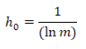
\includegraphics[width=0.2\textwidth]{figures/rumus/5.png}}
	\caption{rumus koefisien}
	\label{rm1}
\end{figure}

diketahui alternatif pada data tersebut sebanyak 3 buah maka nilai koefisien dari rumus tersebut adalah 0,910239227\par
kemudian jika nilai koefisien telah di temukan maka selanjutnya lakukan perkalian nilai yang teelah di normalisasi dengan nilai yang telah dinormalisasi yang dikalikan terlebih dahulu dengan log (ln), untuk lebih jelasnya seperti pada tabel \ref{table8}.
\pagebreak
\begin{table}[h]
\caption{Perkalian nilai normalisasi}
\centering
\begin{tabular}{|c|c|c|c|c|}
\hline
Alternatif & Harga & Kamera & Batrai&Memori\\
\hline
Handphone 1 &(0.222) * ln (0.222) & (0.303) * ln (0.303) & (0.267) * ln (0.267) &  (0.2) * ln (0.2)\\
\hline
Handphone 2 &(0.444) * ln (0.444) & (0.303) * ln (0.303) & (0.467) * ln (0.467)  & (0.4) * ln (0.4)\\
\hline
Handphone 3 &(0.333) * ln (0.333) & (0.393) * ln (0.393) & (0.267) * ln (0.267) &  (0.4) * ln (0.4)\\
\hline

\end{tabular}
\label{table8}
\end{table}

jika telah melakukan perkalian tersebut maka akan mendapatkan hasil, maka dari itu berikut pada tabel \ref{table9} merupakan hasil dari perkalian data yang telah di normalisasi.
\begin{table}[h]
\caption{Data Hasil Kali Nilai Normalisasi}
\centering
\begin{tabular}{|c|c|c|c|c|}
\hline
Alternatif & Harga & Kamera & Batrai&Memori\\
\hline
Handphone 1 &-0,334127293 & -0,361788809 & -0,352575268 & -0,321887582\\
\hline
Handphone 2 &-0,36050 & -0,361788809 & -0,355585952 & -0,366516293\\
\hline
Handphone 3 &-0,366171059 & -0,367040647 & -0,352575268 & -0,366516293\\
\hline
\end{tabular}
\label{table9}
\end{table}

dari data pada tabel \ref{table9} tersebut cari lagi nilai total dari data tersebut, seperti biasa dengan menambahkan nilai dari setiap keriteria namun pada setiap baris ke bawah, bukan menjumlahkan setiap kolom (ke pinggir). 

\begin{table}[h]
\caption{Nilai total data hasil kali}
\centering
\begin{tabular}{|c|c|c|c|}
\hline
 Harga & Kamera & Batrai&Memori\\
\hline
-1,06079559 & -1,090618266 & -1,060736487 &  -1,054920168\\
\hline
\end{tabular}
\label{table10}
\end{table}

jika telah di cari nilai total dari setiap keriteria maka akan menghasilkan hasil seperti pada tabel \ref{table10} tersebut, dikarenakan tadi telah menemukan nilai koefisien dari data tersebut maka kalikan nilai koefisien tersebut dengan nilai total dari setiap keriteria seperti pada tabel \ref{table11} tersebut.

\begin{table}[h]
\caption{nilai total di kali nilai Koefisien}
\centering
\begin{tabular}{|c|c|c|c|}
\hline
 Harga & Kamera & Batrai&Memori\\
\hline
-0,910239227 & -0,910239227 & -0,910239227 &  -0,910239227\\
\hline
* & * & * &  *\\
\hline
-1,06079559 & -1,090618266 & -1,060736487 &   -1,054920168\\
\hline
\end{tabular}
\label{table11}
\end{table}
\pagebreak
kemudian untuk hasil dari perkalian pada tabel \ref{table11} tersebut dapat di lihat pada tabel\ref{table12} berikut ini.

\begin{table}[h]
\caption{Hasil Perkalian Nilai total dengan koefisien}
\centering
\begin{tabular}{|c|c|c|c|}
\hline
 Harga & Kamera & Batrai&Memori\\
\hline
0,965577757 & 0,992723527 &0,96552396 & 0,960229718\\
\hline
\end{tabular}
\label{table12}
\end{table}

jika telah menemukan hasil seperti pada tabel \ref{table12} tersebut maka nilai-nilai tersebut dijadikan pengurang dari nilai 1 (satu), dimana satu tersebut merupakan nilai atau ketentuan dari rumus entropy itu sendiri untuk prosesnya seperti pada tabel \ref {table13}.

\begin{table}[h]
\caption{satu di kurangi hasil perkalian nilai total dengan koefisien}
\centering
\begin{tabular}{|c|c|c|c|}
\hline
 Harga & Kamera & Batrai&Memori\\
\hline
1-0,965577757 &1-0,992723527 &1-0,96552396&1-0,960229718\\
\hline
\end{tabular}
\label{table13}
\end{table}

lalu jika data tersebut telah di kurangkan maka akan mendapatkan hasil seperti pada tabel \ref{table14}
\begin{table}[h]
\caption{Hasil pengurangan}
\centering
\begin{tabular}{|c|c|c|c|}
\hline
 Harga & Kamera & Batrai&Memori\\
\hline
0,034422&0,007276 &0,034476&0,03977\\
\hline
\end{tabular}
\label{table14}
\end{table}
kemudian jika telah mendapatkan hasil seperti pada tabel \ref{table14} lanjutkan dengan menambahkan semua hasil pengurangan tersebut, atau di cari nilai total dari hasil pengurangan tersebut. maka dari itu berikut merupakan hasil nilai total dari hasil pengurangan tersebut.\par

Niali total dari hasil pengurangan tersebut adalah 0,115945

kemudian jika nilai total telah ditemukan maka nilai total tersebut dijadikan pembagi untuk setiap data hasil pengurangan yang terdapat pada setiap keriteria untuk caranya seperti pada tabel \ref{table15} berikut ini 
\begin{table}[h]
\caption{Pembagian nilai total dengan hasil pengurangan}
\centering
\begin{tabular}{|c|c|c|c|}
\hline
 Harga & Kamera & Batrai&Memori\\
\hline
0,034422 /
0,115945
&0,007276
/ 0,115945
&0,034476
/ 0,115945
&0,03977
/ 0,115945
\\
\hline
\end{tabular}
\label{table15}
\end{table}
\pagebreak
dari hasil pembagian tersebut maka akan di hasilkan nilai untuk bobot kriteria atau sering disebut nilai entropy akhir dari setiap keriteria yang mana hasilnya dapat dilihat pada tabel \ref{table16} berikut ini. 

\begin{table}[h]
\caption{Bobot akhir setiap keriteria}
\centering
\begin{tabular}{|c|c|c|c|}
\hline
 Harga & Kamera & Batrai&Memori\\
\hline
0,296884138&0,06275795 &0,29734813&0,343009782\\
\hline
\end{tabular}
\label{table16}
\end{table}

untuk memeriksa apakah nilai bobot tersebut sudah benar maka tinggal tambahkan keseluruhan data bobot dari kriteria maka akan mendapatkan hasil nilai 1 (satu) yang berarti nilai 100\%.

\section{Proses Perhitungan Entropy Ke 2}

Dari Proses perhitungan entropy ke satu niali total dari bobot akan tetap satu walaupun keriteria di tambah menjadi 5 dan seterusnya, untuk membuktikannya brikut merupakan contoh perhitungan entropy ke 2 yang di gunakan untuk membobotkan criteria dari alternatif.\par
	Pada contoh data berikut merupakan contoh data penentuan bobot dari 5(lima) alternatif yaitu yang di misalkan sebagai handphone yang masing-masing memiliki lima keriteria diantaranya terdiri dari Harga (satuan Dolar), kamera depan (tolak ukur pixcel), kamera belakang (tolak ukur pixcel), RAM ( tolak ukur gigabyte (GB)) kapasitas batarai (torakukur mAh), dan Memory penyimpanan ( tolak ukur gigabyte (GB)). Untuk lebih jelasnya berikut merupakan contoh data untuk menentukan bobot criteria.

maka dari itu berikut merupakan data pada tabel \ref{TA1} yang digunakan sebagai bahan untuk perhitungan pada peroses entropy ke 2.


\begin{table}[h]
\caption{Data Handphone dan spesifikasinya 2}
\centering
\begin{tabular}{|c|c|c|c|c|c|}
\hline
\multirow{2}{*}{Alternatif} &\multirow{2}{*}{ Harga}& Kamera & Kamera&\multirow{2}{*}{RAM}& \multirow{2}{*}{Memori}\\
& & depan & belakang & &\\
\hline
Handphone 1 &300& 5 & 24 &  2&64\\
\hline
Handphone 2 &250 & 5 & 13 &  2&32\\
\hline
Handphone 3 &330 & 13 & 24 &  3 &64\\
\hline
Handphone 4 &330 & 5 & 8 &  2 GB&32\\
\hline
Handphone 5 &330 & 2 & 5 &  2 GB&16\\
\hline

\end{tabular}
\label{TA1}
\end{table}

\pagebreak

kemudian dari data pada tabel \ref{TA1} tersebut cari nilai total dari setiap keriteria, jika sudah menemukan nilai total setiap keriteria maka datanya akan seperti pada tabel \ref{TA2} berikut:

\begin{table}[h]
\caption{Nilai Total Setiap Alternatif}
\centering
\begin{tabular}{|c|c|c|c|c|}
\hline
 Harga & Kamera depan & Kamera Belakang&RAM& Memori\\
\hline
1280& 30 & 74 & 11 & 208\\
\hline
\end{tabular}
\label{TA2}
\end{table}

setelah nilai total untuk setiap keriteria di temukan atau didapatkan maka di lanjutkan dengan menormalisasi data dengan menjadikan nilai total dari setiap keriteria tersebut sebagai pembagi untuk setiap data atau nilai yang terdapat pada baris keriteria masing-masing, agar lebh jelas proses pembagian nilainnya seperti pada tabel \ref{TA3} berikut:

\begin{table}[h]
\caption{Normalisasi Data}
\centering
\begin{tabular}{|c|c|c|c|c|c|}
\hline
\multirow{2}{*}{Alternatif} &\multirow{2}{*}{ Harga}& Kamera & Kamera&\multirow{2}{*}{RAM}& \multirow{2}{*}{Memori}\\
& & depan & belakang & &\\
\hline
Handphone 1 &300/1280& 5/30 & 24/74 &  2/11&64/208\\
\hline
Handphone 2 &250/1280 & 5/30 & 13/74 &  2/11&32/208\\
\hline
Handphone 3 &330/1280 & 13/30 & 24/74 &  3/11 &64/208\\
\hline
Handphone 4 &330/1280 & 5/30 & 8/74 &  2/11&32/208\\
\hline
Handphone 5 &330/1280 & 2/30 & 5/74 &  2/11&16/208\\
\hline

\end{tabular}
\label{TA3}
\end{table}

	jika data telah di lakukan pembagian maka akan mendapatkan nilai hasi pembagian, pada tabel \ref{TA4} berikut merupakan hasil dari proses pembagian nilai olen nilai total dari setiap kriteria.

\begin{table}[h]
\caption{Hasil Normalisasi}
\centering
\begin{tabular}{|c|c|c|c|c|c|}
\hline
\multirow{2}{*}{Alternatif} &\multirow{2}{*}{ Harga}& Kamera & Kamera&\multirow{2}{*}{RAM}& \multirow{2}{*}{Memori}\\
& & depan & belakang & &\\
\hline
Handphone 1 &0,234375& 0,166667 & 0,324324 & 0,181818 & 0,307692\\
\hline
Handphone 2 & 0,195313 & 0,166667 & 0,175676 & 0,181818 & 0,153846\\
\hline
Handphone 3 & 0,257813 & 0,433333& 0,324324 & 0,272727 & 0,307692\\
\hline
Handphone 4 & 0,164063 & 0,166667& 0,108108 & 0,181818 & 0,153846\\
\hline
Handphone 5 & 0,148438 & 0,166667& 0,067568 & 0,181818 & 0,076923\\
\hline
\end{tabular}
\label{TA4}
\end{table}

Setelah data selesai di normalisasi dengan hasil data seperti pada tabel \ref{TA4} tersebut maka lanjutkan ke proses persamaan entropy, cari nilai koefisien untuk data tersebut menggunakan rumus koefisien pada gambar \ref{rmm1} berikut:

\begin{figure}[h]
	\centerline{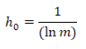
\includegraphics[width=0.2\textwidth]{figures/rumus/5.png}}
	\caption{rumus koefisien}
	\label{rmm1}
\end{figure}

yang dimana pada data tersebut terdapat total jumlah alternatif sebanyak 5 , di karenakan pada data tersebut mempunyai lima alternatif maka nilai koefisien akan menjadi 0,621334935 \par

kemudian jika prosen mencari koefisien telah selesai maka selanjutnya cari nilai antara perkalian nilai yang telah di normalisasi dengan nilai normalisasi yang telah di kalikan dengan Ln (log).agar lebih jelas pada tabel \ref{TA5} berikut merupakan peroses perhitungan perkalian nilai yang telah di normalisasi.
\begin{table}[h]
\caption{Data Handphone dan spesifikasinya 2}
\centering
\begin{tabular}{|c|c|c|c|c|c|}
\hline
\multirow{2}{*}{Alternatif} &\multirow{2}{*}{ Harga}& Kamera & Kamera&\multirow{2}{*}{RAM}& \multirow{2}{*}{Memori}\\
& & depan & belakang & &\\
\hline
\multirow{3}{*}{Handphone 1} & (0,234375) & (0,166667)& (0,324324) &(0,181818) &(0,307692) \\
&* ln  &* ln  &* ln  &* ln  & * ln \\
&(0,234375) & (0,166667) &(0,324324) &(0,181818) &(0,307692)\\
\hline
\multirow{3}{*}{Handphone 2}&(0,195313)&(0,166667&(0,175676) &(0,181818) &(0,153846) \\
&* ln  &* ln  &* ln  &* ln  & * ln \\
&(0,195313)&(0,166667&(0,175676) &(0,181818) &(0,153846)\\
\hline
\multirow{3}{*}{Handphone 3}&(0,257813)&(0,433333) &(0,324324)&(0,272727)&(0,307692)\\
&* ln  &* ln  &* ln  &* ln  & * ln \\
&(0,257813)&(0,433333) &(0,324324)&(0,272727)&(0,307692)\\
\hline
\multirow{3}{*}{Handphone 4}&(0,164063)&(0,166667)&(0,181818)&(0,108108)&(0,153846)\\
&* ln  &* ln  &* ln  &* ln  & * ln \\
&(0,164063)&(0,166667)&(0,108108)&(0,181818)&(0,153846)\\
\hline
\multirow{3}{*}{Handphone 5}&(0,148438)&(0,066667)&(0,067568)&(0,181818)&(0,076923)\\
&* ln  &* ln  &* ln  &* ln  & * ln \\
&(0,148438)&(0,066667)&(0,067568)&(0,181818)&(0,076923)\\
\hline
\end{tabular}
\label{TA5}
\end{table}

kemudian jika perhitungan tersebut telah selesai maka hasilnya akan seperti pada tabel \ref{TA6} berikut ini, kemudian semua nilai yang ada pada tabel tersebut akan dalam keadaan negatif.
\pagebreak
\begin{table}[h]
\caption{Hasil Normalisasi}
\centering
\begin{tabular}{|c|c|c|c|c|c|}
\hline
\multirow{2}{*}{Alternatif} &\multirow{2}{*}{ Harga}& Kamera & Kamera&\multirow{2}{*}{RAM}& \multirow{2}{*}{Memori}\\
& & depan & belakang & &\\
\hline
Handphone 1 &-0,34004& -0,29863 &-0,36519 & -0,30995 & -0,362663\\
\hline
Handphone 2 &-0,31898 & -0,29863 & -0,30552 & -0,30995 & -0,28797\\
\hline
Handphone 3 &-0,34947 & -0,36237& -0,36519 & -0,35435 & -0,362663\\
\hline
Handphone 4 & -0,29654 & -0,29863& -0,2405 &-0,30995 & -0,28797\\
\hline
Handphone 5 &-0,28316 & -0,18054&-0,18207& -0,30995 & -0,197304\\
\hline
\end{tabular}
\label{TA6}
\end{table}

kemudian jika telah mendapatkan hasil seperti pada tabel \ref{TA6} tersebut dilanjutkan dengan mencari nilai total dari setiap keriteria dari tabel \ref{TA6} tersebut, dengan cara menambahkan setiap data keriteria dari data alternatif satu sampai data alternatif terakhir pada data tersebut.

\begin{table}[h]
\caption{Nilai Total Setiap Alternatif}
\centering
\begin{tabular}{|c|c|c|c|c|}
\hline
\multirow{2}{*}{ Harga}& Kamera & Kamera&\multirow{2}{*}{RAM}& \multirow{2}{*}{Memori}\\
& depan & belakang & &\\
\hline
-1,58819& -1,43879 & -1,45848 & -1,59417 & -1,498569\\
\hline

\end{tabular}
\label{TA7}
\end{table}

pada tabel \ref{TA7} merupakan hasil nilai total yang di dapatkan dari tabel \ref{TA6} dimana nilai total terdiri dari lima nilai total dari lima keriteria yaitu nilai tital harga, nilai tital kamera depan, belakang, nilai total RAM dan nilai total Memory.\par

kemudian setelah nilai total di dapatkan lanjutkan dengan mengalikan nilai total tersebut dengan nilai ln atau koefisien yang telah di cari terlebih dahulu, untuk caranya seperti pada tabel \ref{TA8} berikut ini.


\begin{table}[h]
\caption{Perkalian Nilai total dengan LN}
\centering
\begin{tabular}{|c|c|c|c|c|}
\hline
\multirow{2}{*}{ Harga}& Kamera & Kamera&\multirow{2}{*}{RAM}& \multirow{2}{*}{Memori}\\
& depan & belakang & &\\
\hline
-0,62133& -0,62133 & -0,62133 & -0,62133 & -0,62133\\
*-1,58819& *-1,43879 & *-1,45848 & *-1,59417 & *-1,498569\\
\hline
\end{tabular}
\label{TA8}
\end{table}

kemudian untuk hasil perkalian pada tabel\ref{TA8} tersebut dapat dilihat pada tabel \ref{TA9} berikut ini dimana nilai nya menjadi positif, pada hasil tersebut juga dapat di ketahui kenapa nilai koefisien harus negatif atau dalam keadaan negatif hal ini agar bobot awal entropy menjadi positif.
\pagebreak

\begin{table}[h]
\caption{Nilai Bobot Awal Entropy}
\centering
\begin{tabular}{|c|c|c|c|c|}
\hline
\multirow{2}{*}{ Harga}& Kamera & Kamera&\multirow{2}{*}{RAM}& \multirow{2}{*}{Memori}\\
& depan & belakang & &\\
\hline
0,986796& 0,893971 & 0,906202 & 0,990511 & 0,931113\\
\hline

\end{tabular}
\label{TA9}
\end{table}

jika hasil perkalian atau bobot awal entropy telah di dapatkan maka bobot tersebut harus di jadikan sebagai pengurang dari nilai satu, yang dimana satu tersebut sudah ketentuan dari rumus bobot entropy akhir. Agar lebih jelasnya pada tabel \ref{TA10} tersebut merupakan peroses pengurangan nilai satu dengan bobot entropy awal.

\begin{table}[h]
\caption{Pengurangan 1 dengan entropy awal}
\centering
\begin{tabular}{|c|c|c|c|c|}
\hline
\multirow{2}{*}{ Harga}& Kamera & Kamera&\multirow{2}{*}{RAM}& \multirow{2}{*}{Memori}\\
& depan & belakang & &\\
\hline
1-0,986796& 1-0,893971 & 1-0,906202 & 1-0,990511 & 1-0,931113\\
\hline

\end{tabular}
\label{TA10}
\end{table}

Berikut merupakan hasil dari pengurangan pada tabel \ref{TA10}, untuk hasil pengurangannya terdapat pada tabel \ref{TA11} berikut ini:


\begin{table}[h]
\caption{Nilai Total Setiap Alternatif}
\centering
\begin{tabular}{|c|c|c|c|c|}
\hline
\multirow{2}{*}{ Harga}& Kamera & Kamera&\multirow{2}{*}{RAM}& \multirow{2}{*}{Memori}\\
& depan & belakang & &\\
\hline
0,013204&0,106029&0,093798&0,009489&0,068887\\
\hline

\end{tabular}
\label{TA11}
\end{table}

Dari data yang terdapat pada tabel \ref{TA11} tersebut di lakukan penjumlahan untuk semua data tersebut dengan tujuan untuk mencari nilai total dari data tersebut, jika telah di jumlahkan maka akan mendapatkan nilai total dari data tersebut maka dari itu berikut merupakan nilai total dari data tersebut\par

0,291406393

kemudian setelah nilai total tersebut di dapatkan maka nilai total tersebut di jadikan pembagi untuk data yang terdapat pada tabel \ref{TA11} hal ini bertujuan untuk mendapatkan nilai entropy akhir untuk setiap keriteria. kemudian untuk detail pembagian data tersebut dapat di lihat pada tabel \ref{TA12} berikut ini.

\begin{table}[h]
\caption{Nilai Total Setiap Alternatif}
\centering
\begin{tabular}{|c|c|c|c|c|}
\hline
\multirow{2}{*}{ Harga}& Kamera & Kamera&\multirow{2}{*}{RAM}& \multirow{2}{*}{Memori}\\
& depan & belakang & &\\
\hline
0,013204&0,106029&0,093798&0,009489&0,068887\\
/0,291406&/0,291406&/0,291406&/0,291406&/0,291406\\
\hline
\end{tabular}
\label{TA12}
\end{table}

Setelah melakukan pembagian dengan nilai total pada tabel \ref{TA12} tersebut maka akan di dapatkan nilai entropy akhir yang terdapat pada tabel \ref{TA13} berikut ini



\begin{table}[h]
\caption{Nilai Total Setiap Alternatif}
\centering
\begin{tabular}{|c|c|c|c|c|}
\hline
\multirow{2}{*}{ Harga}& Kamera & Kamera&\multirow{2}{*}{RAM}& \multirow{2}{*}{Memori}\\
& depan & belakang & &\\
\hline
0,04531&0,363853&0,321882&0,032561&0,236394\\
\hline

\end{tabular}
\label{TA13}
\end{table}

Pada tabel \ref{TA13} tersebut merupakan nilai entropy akhir, jika di totalkan nilainya akan berjumlah 1, hal ini membuktikan walaupun jumlah keriteria ditambah menjadi banyak maka nilai total akan tetap 1 (satu) yang mana nilai satu akan terbagi sesuai banyaknya kriteria. \par

Dari kedua contoh tersebut dapat dilihat perbedaan yang cukup signifikan yang terdapat pada kriteria harga yang pada contoh ke satu memiliki bobot yang dominan sedangkan pada contoh yang kedua bobot untuk keriteria harga menjadi sangat kecil, begitu pula untuk keriteria kamera pada contoh yang pertama memiliki nilai bobot yang cukup kecil sedangkan pada contoh yang kedua memiliki nilai yang cukup dominan baik itu kriteria kamera depan maupun kamaera belakang.\par

Hal ini membuktikan bahwa tingkat fariasi data yang terdapat pada setiap kriteria sangat berpengaruh untuk lebih jelasnya dapat dilihat pada tabel data untuk contoh ke 1 berikut:

\begin{table}[h]
\caption{Data Handphone dan spesifikasinya 1}
\centering
\begin{tabular}{|c|c|c|c|c|}
\hline
Alternatif & Harga & Kamera & Batrai&Memori\\
\hline
Handphone 1 &1000 & 10 MP & 2000 mAh &  16 GB\\
\hline
Handphone 2 &2000 & 10 MP & 3500 mAh &  32 GB\\
\hline
Handphone 3 &1500 & 13 MP & 2000 mAh &  32 GB\\
\hline

\end{tabular}
\label{T3-1}
\end{table}

Yang di maksud tingkat fariasi data yang terdapat keriteria yaitu perubahan data atau jenis data yang terdapat pada keriteria misalkan pada keriteria Harga pada tebel tersebut ternyata nilai untuk keriteria tersebut memiliki pola yaitu kelipatan dari 5 begitu pula pada keriteria batrai juga memiliki pola dan juga kriteria memori. Sedangkan kenapa suatu keriteria bisa memiliki bobot yang kecil di karenakan data pada keriteria tersebut acak seperti pada kriteria kamera pada tabel tersebut. \par

Selain kedua hal tersebut hal yang dapat memperbesar bobot kriteria secara signifikan yaitu data yang acak tetapi memiliki jarak yang sangat jauh sepeerti pada keriteria kamera ada nilai 2 dan 24 maka keriteria tersebut kemungkinan memiliki bobot yang sangat besar.\par

Kemudian bagaimana cara mengatasi hal tersebut, agar pembagian bobot bisa sesuai dan tidak terlalu membingungkan bagi pengambil keputusan bisa dilakukan cara mengkalsifikasikan data data tersebut, lantas bagaimana cara mengkalsifikasikan data tersebut misalkan data yang terdapat pada stu keriteria ternyata memiliki pola yaitu data paling kecil merupakan 1 dan data paling besar merupakan 50 bisa di klasifikasikan menjadi 5 data lain dengan nilai 1 – 5 atau bisa diklasifikasikan datanya dari 1 sampai 9 untuk contohnya seperti berikut.\par

Misalkan data yang terdapat pada keriteria ke satu memiliki nilai antara 1 sampai 50 maka di bagi menjadi nilai tersebut misalkan menjadi 5 klasifikasi atau bisa di sebut sub keriteria misalkan pembagiannya seperti berikut:

\begin{enumerate}
\item Jika nilai pada kriteria1 diantara 1 sampai 10 maka memiliki nilai atau bobot 1 (satu)

\item Jika nilai pada kriteria1 diantara 11 sampai 20 maka memiliki nilai atau bobot 2 (dua)

\item Jika nilai pada kriteria1 diantara 21 sampai 30 maka memiliki nilai atau bobot 3 (dua)

\item Jika nilai pada kriteria1 diantara 31 sampai 40 maka memiliki nilai atau bobot 4 (dua)

\item Jika nilai pada kriteria1 diantara 41 sampai 50 maka memiliki nilai atau bobot 5 (dua)

\end{enumerate}

Atau untuk lebih sederhananya seperti pada tabel \ref{TB} berikut:

\begin{table}[h]
\caption{Aturan untuk menghimpun data}
\centering
\begin{tabular}{|c|c|c|c|c|}
\hline
Aturan & Bobot atau nilai \\
\hline
1 ≤ X ≤ 10 &1\\
\hline
11 ≤ X ≤ 20 &2\\
\hline
21 ≤ X ≤ 30 &3\\
\hline
31 ≤ X ≤ 40 &4\\
\hline
41 ≤ X ≤ 50 &5\\
\hline

\end{tabular}
\label{TB}
\end{table}

Cara klasifikasi ini dapat diterapkan untuk mencari entropy namun untuk penggunaanya harus disesuaikan dengan keadaan dan keperluan pengambil keputusan sehingga dapat menghasilkan bobot yang sesuai untuk keriteria, kemudian untuk nilai 1 sampai 50 pada contoh tersebut hanya perumpamaan agar mendapat gambaran untuk memecahkan permasalahan yang mirip seperti kasus tersebut.
\pagebreak
\section{Proses Perhitungan Entropy Ke 3}

Pada contoh atau preoses perhitungan ke 3 ini akan di bahas cara mengklasifikasikan data sebagai solusi dari jenus data yang tingkat fariasinya sangat tinggi, maka dari itu pada perhitungan ke tiga ini menggunakan data siswa dengan nilai sebagai keriterianya.

dimana untuk data keriteria yang di gunakan pada contoh ini adalah sebagai berikut:

\begin{enumerate}
\item Nilai Matematika (MTK)
\item Nilai IPS
\item Nilai IPA
\item Nilai Bahasa Indonesia (BI)
\end{enumerate}

adapun nilai yang terdapat pada setiap keriteria antara nol (0) sampai dengan seratus (100)\par

sedangkan untuk data yang akan diolah terdapat pada tabe \ref{ts1} berikut:

\begin{table}[h]
\caption{Data Nilai Siswa}
\centering
\begin{tabular}{|c|c|c|c|c|}
\hline
Alternatif & MTK & IPS & IPA&BI\\
\hline
Siswa 1 &92 & 70 & 88 &  65\\
\hline
Siswa 2 &70 & 80 & 58 &  76\\
\hline
Siswa 3 &83 & 60 & 75 &  80\\
\hline
Siswa 4 &60 & 87 & 67 &  60\\
\hline
Siswa 5 &55 & 89 & 76 &  87\\
\hline

\end{tabular}
\label{ts1}
\end{table}

yang dimana untuk mengolah data tersebut terdapat aturan klasifikasi yang mengambil nilai terkecil yaitu satu (1) kemudian untuk nilai terbesar yaitu lima (5) adapun aturan untuk klasifikasi data tersebut adalah sebagai berikut:

\begin{enumerate}
\item Jika niali antara 0 – 20 memiliki bobot atau nilai samadengan 1 (satu)
\item Jika niali antara 21 – 40 memiliki bobot atau nilai samadengan 2 (dua)
\item Jika niali antara 41 – 60 memiliki bobot atau nilai samadengan  3 (tiga)
\item Jika niali antara 61 – 80 memiliki bobot atau nilai samadengan 4 (empat)
\item Jika niali antara 81 – 100 memiliki bobot atau nilai samadengan 5 (lima)
\end{enumerate}
\pagebreak
	Aturan tersebut berlaku untuk semua keriteria, jika keriteria tersebut tidak memiliki varian data yang mirip atau sama maka dianjurkan untuk setiap keriteria aturan di buat berbeda.\par

kemudian data yang terdapat pada tabel \ref{ts1} di normalisasi sesuai dengan aturan yang telah di buat,pada tabel \ref{ts2} berikut ini merupakan data hasil normalisasi:

\begin{table}[h]
\caption{Data Nilai Siswa}
\centering
\begin{tabular}{|c|c|c|c|c|}
\hline
Alternatif & MTK & IPS & IPA&BI\\
\hline
Siswa 1 &5 & 4 & 5 &  4\\
\hline
Siswa 2 &4 & 4 & 3 &  4\\
\hline
Siswa 3 &5 & 3 & 4 &  4\\
\hline
Siswa 4 &3 & 5 & 4 &  3\\
\hline
Siswa 5 &3 & 5 & 4 &  5\\
\hline
\end{tabular}
\label{ts2}
\end{table}

Setelah data didapatkan seperti pada tabel \ref{ts2} tersebut baru kemudian data tersebut bisa di olah atau di lakukan proses entropy untuk peroses entropy sama dengan proses entropy pada perhitungan entropy  ke 1 dan perhitungan entropy ke 2.

pada langkah pertama cari nilai total dari setiap keriteria, pada tabel \ref{ts3} berikut merupakan nilai total dari setiap keriteria:

\begin{table}[h]
\caption{Nilai Total Kriteria}
\centering
\begin{tabular}{|c|c|c|c|c|}
\hline
 MTK & IPS & IPA&BI\\
\hline
20 & 21 & 20 &  20\\
\hline
\end{tabular}
\label{ts3}
\end{table}

setelah mendapatkan nilai total dari setiap keriteria jadikan nilai total tersebut menjadi pembagi untuk masing masing nilai keriteria, untuk lebih jelasnya seperti pada tabel \ref{ts4} berikut:


\begin{table}[h]
\caption{Normalisasi Data Nilai Siswa}
\centering
\begin{tabular}{|c|c|c|c|c|}
\hline
Alternatif & MTK & IPS & IPA&BI\\
\hline
Siswa 1 &5/20 & 4/21 & 5/20 &  4/20\\
\hline
Siswa 2 &4/20 & 4/21 & 3/20 &  4/20\\
\hline
Siswa 3 &5/20 & 3/21 & 4/20 &  4/20\\
\hline
Siswa 4 &3/20 & 5/21 & 4/20 &  3/20\\
\hline
Siswa 5 &3/20 & 5/21 & 4/20 &  5/20\\
\hline
\end{tabular}
\label{ts4}
\end{table}
\pagebreak
jika sudah selesai membagikan nilai keriteria dengan nilai total setiap keriteria maka akan mendapatkan hasi dari pembagian seperti pada tabel \ref{ts5} berikut ini:


\begin{table}[h]
\caption{Data Hasil Normalisasi}
\centering
\begin{tabular}{|c|c|c|c|c|}
\hline
Alternatif & MTK & IPS & IPA&BI\\
\hline
Siswa 1 &0,25 & 0,19047619 & 0,25 &  0,2\\
\hline
Siswa 2 &0,2 & 0,19047619 & 0,15 &  0,2\\
\hline
Siswa 3 &0,25 & 0,142857143 & 0,2 &  0,2\\
\hline
Siswa 4 &0,15 & 0,238095238 & 0,2 &  0,15\\
\hline
Siswa 5 &0,15 & 0,238095238 & 0,2 &  0,25\\
\hline
\end{tabular}
\label{ts5}
\end{table}

Setelah data selesai di normalisasi dengan hasil data seperti pada tabel \ref{ts5} tersebut maka lanjutkan ke proses persamaan entropy, cari nilai koefisien untuk data tersebut menggunakan rumus koefisien pada gambar \ref{rmmm1} berikut:

\begin{figure}[h]
	\centerline{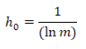
\includegraphics[width=0.2\textwidth]{figures/rumus/5.png}}
	\caption{rumus koefisien}
	\label{rmmm1}
\end{figure}

yang dimana pada data tersebut terdapat total jumlah alternatif sebanyak 5 , di karenakan pada data tersebut mempunyai lima alternatif maka nilai koefisien akan menjadi \par

0,621334935 \par
\pagebreak
kemudian jika prosen mencari koefisien telah selesai maka selanjutnya cari nilai antara perkalian nilai yang telah di normalisasi dengan nilai normalisasi yang telah di kalikan dengan Ln (log).agar lebih jelas pada tabel \ref{ts6} berikut merupakan peroses perhitungan perkalian nilai yang telah di normalisasi.


\begin{table}[h]
\caption{Data perkalian nilai normalisasi}
\centering
\begin{tabular}{|c|c|c|c|c|}
\hline
Alternatif & MTK & IPS & IPA&BI\\
\hline
\multirow{3}{*}{Siswa 1} & (0,25) & (0,19047619)& (0,25) &(0,2)\\
&* ln  &* ln  &* ln  &* ln \\
&(0,25) & (0,19047619) &(0,25) &(0,2)\\
\hline
\multirow{3}{*}{Siswa 2}&(0,2)&(0,19047619)&(0,15) &(0,2)\\
&* ln  &* ln  &* ln  &* ln \\
&(0,2)&(0,19047619)&(0,15) &(0,2)\\
\hline
\multirow{3}{*}{Siswa 3}&(0,25)&(0,142857143) &(0,2)&(0,2)\\
&* ln  &* ln  &* ln  &* ln\\
&(0,25)&(0,142857143) &(0,2)&(0,2)\\
\hline
\multirow{3}{*}{Siswa 4}&(0,15)&(0,238095238)&(0,2)&(0,15)\\
&* ln  &* ln  &* ln  &* ln\\
&(0,15)&(0,238095238)&(0,2)&(0,15)\\
\hline
\multirow{3}{*}{Siswa 5}&(0,15)&(0,238095238)&(0,2)&(0,25)\\
&* ln  &* ln  &* ln  &* ln\\
&(0,15)&(0,238095238)&(0,2)&(0,25)\\
\hline
\end{tabular}
\label{ts6}
\end{table}


jika proses perkalian tersebut telah selesai maka akan mendapatkan hasil brupa bilangan minus, untuk hasil perkalian tersebut dapat di lihat pada tabel \ref{ts7}

\begin{table}[h]
\caption{Data Hasil Perkalian normalisasi}
\centering
\begin{tabular}{|c|c|c|c|c|}
\hline
Alternatif & MTK & IPS & IPA&BI\\
\hline
Siswa 1 &-0,34657359 & -0,315852967 & -0,34657359 &  -0,321887582\\
\hline
Siswa 2 &-0,321887582 & -0,315852967 & -0,284567998 & -0,321887582\\
\hline
Siswa 3 &-0,34657359 & -0,277987164 & 0,321887582 & -0,321887582\\
\hline
Siswa 4 &-0,284567998 &-0,341686792 & 0,321887582 & -0,284567998\\
\hline
Siswa 5 &-0,284567998 &- 0,341686792 & 0,321887582 & -0,34657359\\
\hline
\end{tabular}
\label{ts7}
\end{table}

jika semua hasil dari perkalian tersebut telah di temukan maka langkah selanjutnya yaitu mencari nilai total dari hasil perhitungan tersebut yaitu pada tabel \ref{ts7} kemudian untuk hasil nilai totalnya yaitu dapat di lihat pada tabel \ref{ts8} berikut ini
\pagebreak
\begin{table}[h]
\caption{Nilai Total hasil kali normalisasi}
\centering
\begin{tabular}{|c|c|c|c|c|}
\hline
 MTK & IPS & IPA&BI\\
\hline
-1,584170759 & -1,593066682 & -1,596804335 &  -1,596804335\\
\hline
\end{tabular}
\label{ts8}
\end{table}

kemudian jika data nilai total telah di temukan lanjutkan dengan perkalian, dimana nilai total tersebut di kalikan dengan nilai koefisien yang telah di temukan di hitung sebelumnya, untuk detail perhitungannya dapat di lihat pada tabel \ref{ts9} berikut ini:


\begin{table}[h]
\caption{Perkalian nilai koefisien dengan nilai total}
\centering
\begin{tabular}{|c|c|c|c|c|}
\hline
 MTK & IPS & IPA&BI\\
\hline
-0,621334935&-0,621334935&-0,621334935&-0,621334935\\
*&*&*&*\\
-1,584170759 & -1,593066682 & -1,596804335 &  -1,596804335\\
\hline
\end{tabular}
\label{ts9}
\end{table}

kemudian untuk hasil dari perkalian tersebut seperti pada tabel \ref{ts10} berikut ini:

\begin{table}[h]
\caption{Hasil Perkalian nilai koefisien dengan nilai total}
\centering
\begin{tabular}{|c|c|c|c|c|}
\hline
 MTK & IPS & IPA&BI\\
\hline
0,984300635&0,989827982&0,992150317&0,992150317\\
\hline
\end{tabular}
\label{ts10}
\end{table}

kemudian hasil perkalian pada tabel \ref{ts10} tersebut dijadikan pengurang dari satu (1) dimana nilai satu tersebut di dapatkan dariketentuan rumus untuk mencari nilai entropy akhir sehingga pada tahapan selanjutnya nilai hasil perkalian tersebut di jadikan pengurang, untuk lebih jelasnya seperti pada tabel \ref{ts11} berikut ini:


\begin{table}[h]
\caption{Pengurangan data dengan nilai satu}
\centering
\begin{tabular}{|c|c|c|c|c|}
\hline
 MTK & IPS & IPA&BI\\
\hline
1-0,984300635&1-0,989827982&1-0,992150317&1-0,992150317\\
\hline
\end{tabular}
\label{ts11}
\end{table}
jika sudah di kurangkan maka akan mendapatkan hasil seperti pada tabel \ref{ts12} berikut ini:


\begin{table}[h]
\caption{Hasil Pengurangan data dengan nilai satu}
\centering
\begin{tabular}{|c|c|c|c|c|}
\hline
 MTK & IPS & IPA&BI\\
\hline
0,015699365&0,010172018&0,007849683&0,007849683\\
\hline
\end{tabular}
\label{ts12}
\end{table}
\pagebreak
Dari data yang terdapat pada tabel \ref{ts12} tersebut di lakukan penjumlahan untuk semua data tersebut dengan tujuan untuk mencari nilai total dari data tersebut, jika telah di jumlahkan maka akan mendapatkan nilai total dari data tersebut maka dari itu berikut merupakan nilai total dari data tersebut\par

0,041570749

kemudian setelah nilai total tersebut di dapatkan maka nilai total tersebut di jadikan pembagi untuk data yang terdapat pada tabel \ref{ts12} hal ini bertujuan untuk mendapatkan nilai entropy akhir untuk setiap keriteria. kemudian untuk detail pembagian data tersebut dapat di lihat pada tabel \ref{ts13} berikut ini.

\begin{table}[h]
\caption{Hasil Pengurangan data dengan nilai satu}
\centering
\begin{tabular}{|c|c|c|c|c|}
\hline
 MTK & IPS & IPA&BI\\
\hline
0,015699365&0,010172018&0,007849683&0,007849683\\
/ 0,041570749&/ 0,041570749&/ 0,041570749& / 0,041570749\\
\hline
\end{tabular}
\label{ts13}
\end{table}

Kemudian untuk hasil dari pembagian pada tabel \ref{ts13} tersebut, terdapat pada tabel \ref{ts14} berikut ini:

\begin{table}[h]
\caption{Nilai Entropy Akhir}
\centering
\begin{tabular}{|c|c|c|c|c|}
\hline
 MTK & IPS & IPA&BI\\
\hline
0,377654144&0,244691713&0,188827072&0,188827072\\
\hline
\end{tabular}
\label{ts14}
\end{table}
pada tabel tersebut merupakan data bobot entropy akhir yang jika di totalkan maka akan mendapatkan nilai satu (1) yang berarti bobot dari criteria tersebut hasil pembagian dari nilai 1, nilai satu tersebut bisa di anggap 100\%.

\pagebreak

\textbf{Catatan :}\par
\textit{Untuk perhitungan entropy yang ke 3 untuk aturannya dapat di padukan atau di kolaborasikan dengan metode lain, karena banyak metode yang di gunakan untuk sorting data atau mengklasifikasikan data contoh metode fuzzy yang sering dikolaborasikan dengan metode entropy ini, dimana dengan aturan fuzzy data di bagi kemudian di berikan nilai kemudian pada tahapan selanjutnya dengan menggunakan metode entropy di lakukan pencarian bobot sesuai dengan nilai fuzzy yang sudah di hasilkan.}



